\documentstyle[12pt,epsfig]{book}
\title{IBMlib concept description}

\begin{document}

\maketitle  

\tableofcontents

\section{Unresolved issues}

\begin{itemize}

  \item How should we include Kritins algorithms ?

  
\end{itemize}

%%%%%%%%%%%%%%%%%%%%%%%%%%%%%%%%%%%%%%%%%%%%%%%%%%%%%%%%%%%%%%%%%%%%%%%%%%5
\part{User guide }

\chapter{Overall concepts}

IBMlib is a particle simulation toolbox intended research purposes.
The core vision of IBMlib is to provide a light weight environment
that easily allows to combine existing/new biological modules with 
existing/new physical data sets.
IBMlib provides and supports simple core functionality and provides
templates for developments.
The IBMlib implementation concept is shown in Figure \ref{IBMlib:concept}
% ----------------------------------------------------------------------------
\begin{figure}[p]   % [tbhp]
\begin{center}                                                  %% NO_WC_WOUNT
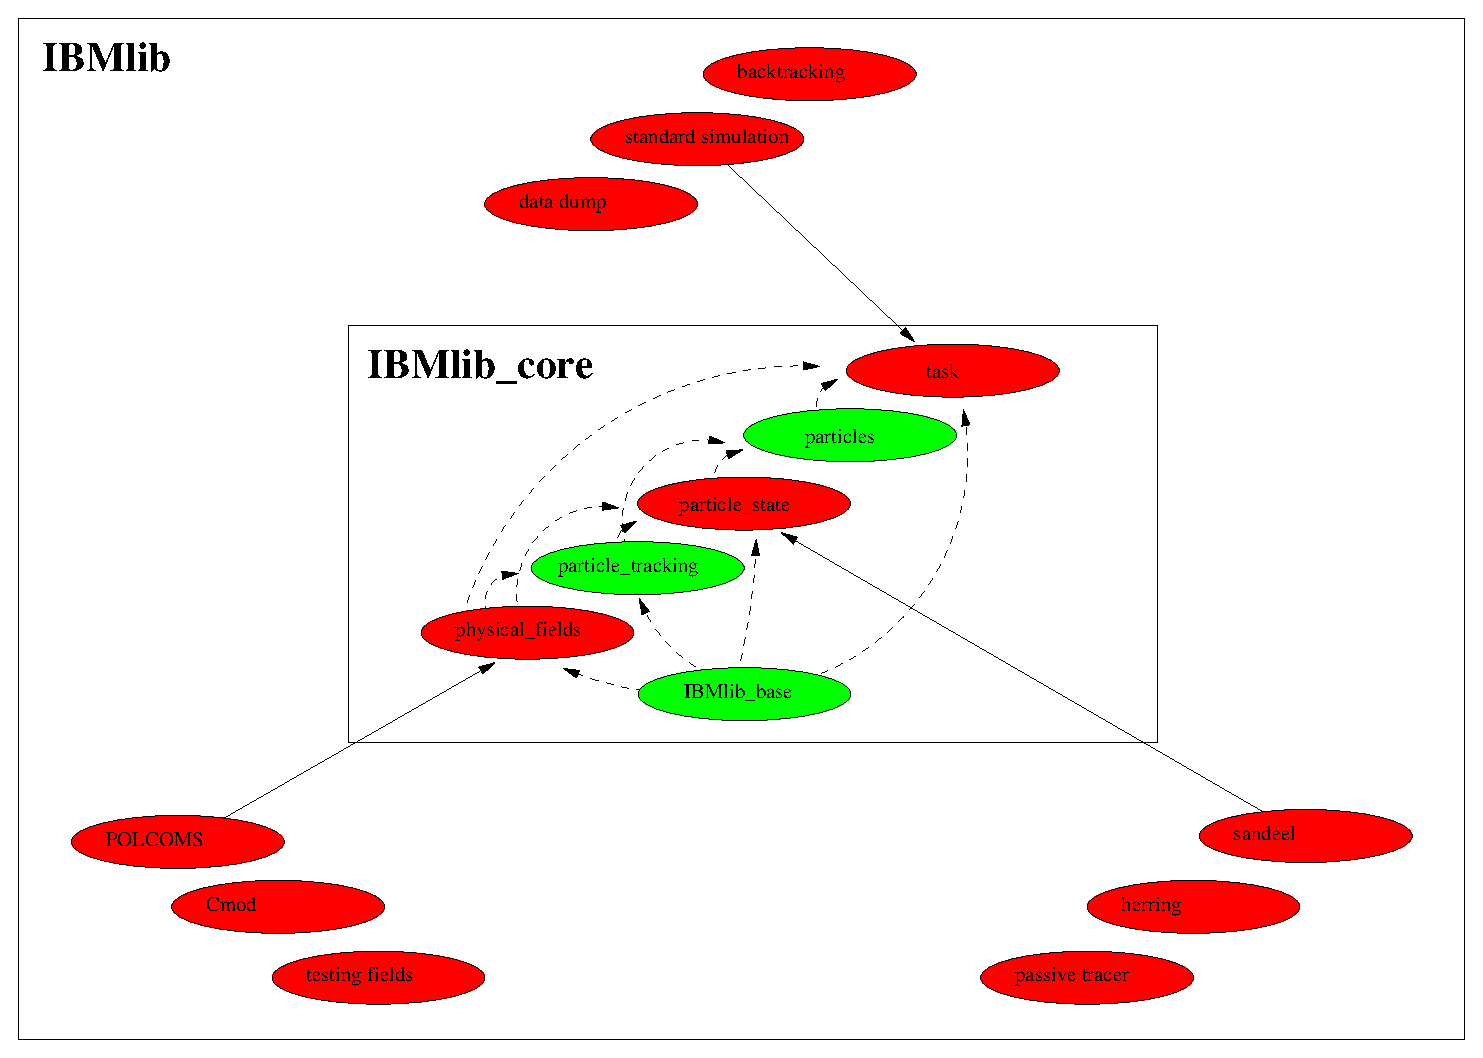
\epsfig{file=IBMlib_module_dependences.eps,width=120mm,angle=0,clip=}     %% NO_WC_WOUNT
%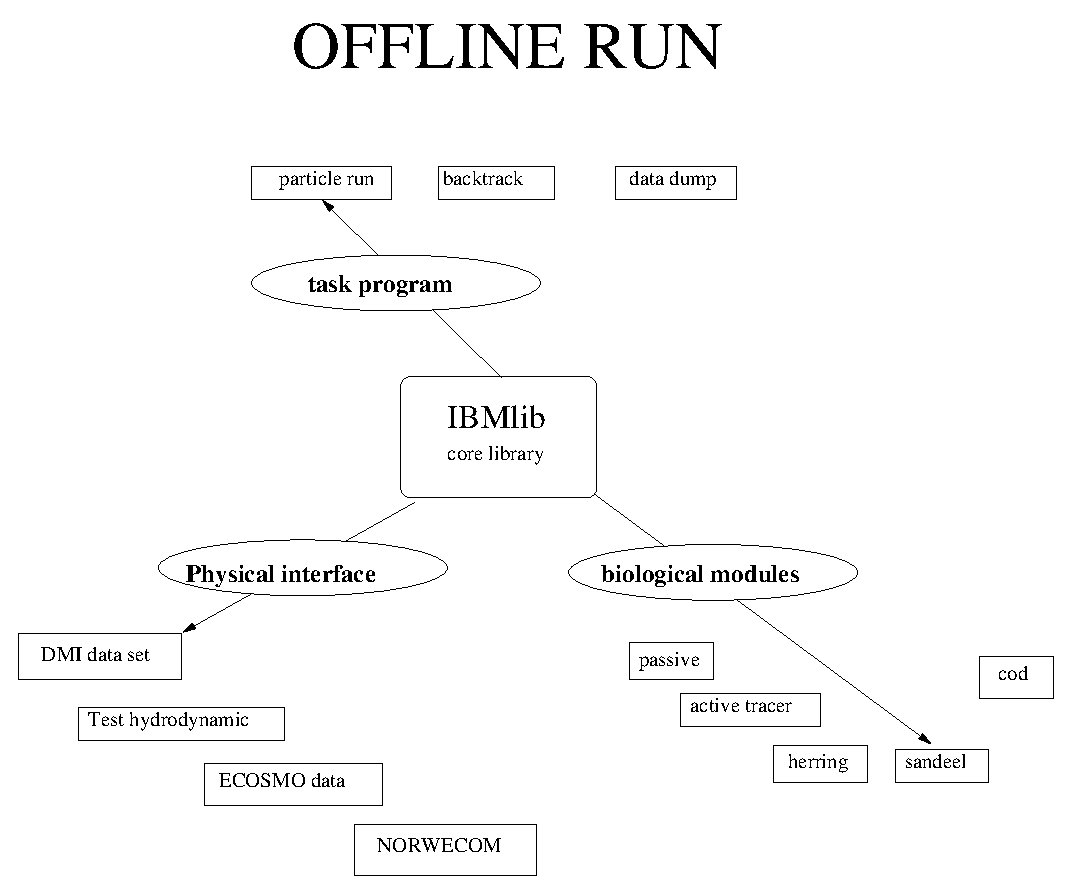
\includegraphics[width=120mm]{IBMlib_offline.eps}     %% NO_WC_WOUNT
\end{center}                                                    %% NO_WC_WOUNT
\caption{Concept diagram of the IBMlib framework.}
\label{IBMlib:concept}
\end{figure}
% ----------------------------------------------------------------------------
It shows a core part IBMlib\_core that contains generic core functionality for
particle tracking. IBMlib\_core accesses the physical environment via the
physical interface; this interface can be linked to any data source that is
able to access the physical environment. The biological properties is specified in 
particle state module that provides the particle state interface to IBMlib; 
this amounts to specifying e.g. how biological tracer grow and swim, if relevant.
The particle state module can also describe passive particles and other 
idealized types. Finally the task interface contrals what IBMlib is actually going 
to do, e.g. a forward simulation or a data dump or any customized run type.
Alltogether, IBMlib\_core and optional modules for physical environment, biological 
properties and tasks constitutes IBMlib; when an actual physical, biological 
and task has been selected, we refer to it as an IBMlib configuration.

online/offline mode

\chapter{License issues}

currently none, likely GPL in future

\chapter{Installation}

\section{System resources and requirements}

IBMlib is currently set up to a Linux environment, however
there should be no fundamental problems to port IBMlib to
other OS environments.

\section{System resources and requirements}

\begin{itemize}
  \item Fortran 90 compiler. All performance code is written in Fortran 90.
  \item Gmake. All makefiles are written for and tested on gmake; other
        make implementations may be used, but this may require 
        minor adaptation to makefiles
  \item Python. Fortran modules are scanned for use associations with a 
        preprocessor utility in Python. At some point we may ship 
        dependency files along to avoid this requirement.

\end{itemize}
Depending on which sub modules for physical environment, biological
properties and tasks constitutes are selected additional system resources
may be required (e.g. NetCDF and HDF) - this should be available from the 
automatic documentation of the sub modules.

\section{Configuration}

You configure IBMlib by selecting sub modules for physical environment, biological
properties and task. In the Makefile, look for make variables
{\tt PHYSICAL\_FIELDS\_DIR,  PARTICLE\_STATE\_DIR,  TASK\_DIR} and point these
to the directories corresponding to the desired sub modules. 

By default, the offline version builds into the executable {\tt  ibmrun}; if you want it
to be called something else, set the make variable {\tt EXECUTABLE} as desired   

\section{Building an IBMlib configuration} 

When the makefile is configured, you simply type
[ make
]
on the command line, which produces and executable {\tt ibmrun} 
(or another target name specified in make variable {\tt EXECUTABLE}).
This executable may be copied to somewhere in the standard executable search PATH, if
it should be installed as an application.

\section{Running an IBMlib configuration}

When the executable is build, you simply type
[ ibmrun [<arguments>]
]
on the command line. Often a file with simulation parameters is required 
as argument after ibmrun; the task sub modules should document which arguments 
and options they require and support.

\section{Simulation files}

When IBMlib is used in a standard task configuration, it expects you 
to provide an input file on the command line like
[ ibmrun <inputfile> [ >  <outputfile>]
]
All parts of the compiled IBMlib configuration will try to 
read most input data from this file in a standard task configuration.
Reading is distributed, meaning that different parts of IBMlib
reads this file independently of the other parts.
The simulation input file is based on
a tagged input ASCII format containing lines as 
\begin{equation}
tag = value [value*] \nonumber
\end{equation}
tag is a character identifier terminated at first occurence of 
the separator $=$. value of the tag is what follows the separator to the end of that 
line and anything can appear here. If the value is a vector, each item in the vector
is separated by spaces (but stay on same line).
IBMlib does not check that all parameters are read.
The same tag may appear many several times - e.g. a particle emission box,
in other cases the tag should be unique, e.g. the patricle time step. In this case
the first occurence is picked, the rest is ignored.
The following rules also apply for the markup:
\begin{itemize}
  \item Comments: everything after (and including) " !" is skipped
  \item Empty lines and spaces:   just ignored
  \item Malformed lines: just ignored (e.g. if you forgot "=")
  \item Everything after "=" is considered part of the value for tag
  \item Required tag (or value) is missing. This will generate a runtime
        error, SLAM will stop, unless a default applied to the tag.
  \item Order of tags does not matter. 
\end{itemize}  

This input format is convenient for scripting, where upper-level  
scripts generates input files. The input is read once
when the simulation is started.
The following are mandatory input parameters:

\subsection{Task = basic\_simulation tags}
\begin{itemize}
  \item {\em start\_time}. The beginning of the simulation, specified as (year  month  day  second\_of\_day)
  \item {\em end\_time}. The end time of the simulation, specified as (year  month  day  second\_of\_day) 
  \item {\em particle\_time\_step}. Nominel time step for the integration algortihm 
        in seconds.
  \item {\em emitbox}. Gives a window in space and time, where sandeel larvae/eggs are released.
        The may be specified as many emitbox entries as desired, in this way they
        may act in parallel and quite complex release patterns can be set up.
        The first 4 integers are (year  month  day  second\_of\_day) where the release
        begins (of that box); the next 4 integers are (year  month  day  second\_of\_day) where the release
        stops (of that box). 
        The next six numbers specify a spatial box (in latitude and longitude) where
        sandeel larvae/eggs are released. Dry (land-locked) sectors of the spatial box are omitted when
        releasing larvae/eggs. The first three numbers are the spatial lower SW corner of the release box
        given as (longitude,latitude,vertical position), the next three numbers are the spatial upper 
        NE corner of the release box given as (longitude,latitude,vertical position).
        The vertical position can be spcified as absolute depth (counted negative below the water surface)
        or as relative depth $z$:$ 0 < z < 1$. 
        $z=0$ corresponds to the sea surface, 
        $z=1$ corresponds to the sea bed.
        Biological particles are released uniformly in time and space with in space-time window
        specified, so that the total number of particles released adds up to the integer given as 
        number 15. All other parameters following number 15 in emit box are passed to the biological module.
        There can be an "e", which means sandeel eggs are released by this emitbox; the can be an "l"
        which means sandeel larvae are released by this emitbox - in the latter case, a number giving 
        the inital length (in mm) of the released sandeel larvae should be provided.
\end{itemize}
\subsection{Particle\_tracking module}
\begin{itemize}
  \item {\em advec\_intg\_method}. The integration algortihm for time forward integration
        of advected sandeel larvae (options are euler (Euler forward) or rk2/rk4 (Runge-Kutta 2 or 4)).
\end{itemize}

\subsection{Example on minimal input file}
{\small 
\begin{verbatim}

!--------------------------------------------
!        Main simulation control file 
!--------------------------------------------

start_time  = 2005 03 01 0    !  year  month  day  second_of_day
end_time    = 2005 03 18 0    !  year  month  day  second_of_day

advec_intg_method  = euler    !  advection scheme: euler/rk2/rk4
particle_time_step = 1800     !  in seconds for time integration of motion

! --------------- biology spatial control ---------------
! r(1:4) start:  year month day sec_of_day
! r(5:8) end:    year month day sec_of_day
! r(9:11)        lon_min lat_min z_min  (z=0 -> surface)
! r(12:14)       lon_max lat_max z_max  (z=1 -> bottom)
! r(15)          max_number_of_tracers
! r(16:)         other input item to particle state

emitbox = 2005 03 02 0     2005 03 02 3600  2 54 1   3 55 1  100 e 
emitbox = 2005 03 02 3600  2005 03 02 7200  4 54 1   5 56 1  100 l 9.66
! -------------------------------------------------------
\end{verbatim}
}

There may be other mandatory entries, depending on which 
oceanography provider and biology provider you are applying in your 
configuration - consult these to find out which input fields are mandatory.

%%%%%%%%%%%%%%%%%%%%%%%%%%%%%%%%%%%%%%%%%%%%%%%%%%%%%%%%%%%%%%%%%%%%%%%%%%

\part{Programmers guide}


\chapter{Makefiles and build protocols}


IBMlib has six dependency levels
\begin{enumerate}
  \item TASK 
  \item particles.mod
  \item PARTICLE\_STATE 
  \item particle\_tracking.mod
  \item PHYSICAL\_FIELDS 
  \item IBMLIB\_BASE (incl. included external tools)  
\end{enumerate}
which gives the allowed use associations (higher to lower or same level) 
and the appropriate build order (from below and up).
One level is only allowed to build objects at its own level (distributed makefiles)
To build an IBMlib configuration, four make files are required:
\begin{enumerate}
  \item Makefile:     
  \item \$(PHYSICAL\_FIELDS\_DIR)/Makefile
  \item \$(PARTICLE\_STATE\_DIR)/Makefile  
  \item \$(TASK\_DIR)/Makefile          
\end{enumerate}
The first is generic and takes care of the overall build syncrinization.
The remaining make files are independent and invoked from the first makefile.
They are not included, because this breaks encapsulation and creates
name clashes. 
The specification of the last three makefiles are given below.
Each makefile of may PHYSICAL\_FIELDS/PARTICLE\_STATE/TASK 
- or may not - include {\tt common.mk}

% --------------------------------------------------------
\section{\$(PHYSICAL\_FIELDS\_DIR)/Makefiles }

Module PHYSICAL\_FIELDS, rooted in PHYSICAL\_FIELDS\_DIR. In this directory, there
should be a makefile updating the targets:
\begin{itemize}
  \item physical\_fields.mod (F90 module interface, in directory PHYSICAL\_FIELDS\_DIR)
  \item physical\_fields.a   (all compiled objects of module, in directory PHYSICAL\_FIELDS\_DIR)
  \item clean
\end{itemize}
An (optional) makefile link\_opt.mk in PHYSICAL\_FIELDS\_DIR may define the following 
variables for link options to be used for the final stage linking:
\begin{itemize}
  \item LINKFLAGS\_PHYSICAL
  \item LINKLIBS\_PHYSICAL 
\end{itemize}

% --------------------------------------------------------
\section{\$(PARTICLE\_STATE\_DIR)/Makefiles }

  
Module PARTICLE\_STATE rooted in PARTICLE\_STATE\_DIR. In this directory, there
should be a makefile updating the targets:
\begin{itemize}
  \item particle\_state.mod (F90 module interface, in directory PARTICLE\_STATE\_DIR)
  \item particle\_state.a   (all compiled objects of module, in directory PARTICLE\_STATE\_DIR)
  \item clean 
\end{itemize}  
An (optional) makefile link\_opt.mk in PARTICLE\_STATE\_DIR may define the following 
variables for link options to be used for the final stage linking:
\begin{itemize}
  \item LINKFLAGS\_STATE
  \item LINKLIBS\_STATE
\end{itemize}  

% --------------------------------------------------------
\section{\$(TASK\_DIR)/Makefiles }

Module TASK rooted in TASK\_DIR  In this directory, there
should be a makefile updating the targets:
\begin{itemize}
  \item task.a (all compiled objects INCLUDING the main program, in directory PARTICLE\_STATE\_DIR)
  \item  clean
\end{itemize}  
An (optional) makefile link\_opt.mk in PHYSICAL\_FIELDS\_DIR may define the following 
variables for link options to be used for the final stage linking:
\begin{itemize}
  \item  LINKFLAGS\_TASK
  \item  LINKLIBS\_TASK    
\end{itemize}  
 

% --------------------------------------------------------
\section{Miscellaneous building notes} 

About order of objects at linking: "The traditional behavior of linkers is to search 
for external functions from left to right in the libraries specified on the command line. 
This means that a library containing the definition of a function should appear after any 
source files or object files which use it ...When several libraries are being used, 
the same convention should be followed for the libraries themselves."

ifort note: apparently this problem with ifort can just be handled
by duplicating link objects once ...


% ============================================================================
\chapter{Data stractures, variables and units}

\section{Space}
  Space in IBMlib is continuous and {\em grid free} and data
  is accessed by query functions; thereby grid details
  (grid type, resoultion, nested grids, vertical layer structure, layout etc) are
  hidden behind the physical interface and the 
  particle ware code becomes independent of particular 
  data sets.

\subsection{Space units}  \label{Spaceunits}
  At the particle side horizontal coordinates $(x,y)$ are 
  longitude (degrees East) and latitude (degrees North) and
  vertical coordinate $z$ is depth below actual sea surface in meters
  (i.e. positive down, zero at actual sea surface).

\subsection{Vector orientation and units }    \label{Vectororientationandunits}
  At the particle side vectors are oriented along tangent space 
  vectors in appropriate units. This means that vectors pointing East and North
  are positive and the positive vertical direction is toward the bottom. 
  Note that this means that unit vectors for (longitude,latitude,vertical) 
  (in this order) forms a left hand screw; we think it is more convenient
  to have water depth positive with zero at surface than forming a right hand screw.
  Behind the interface(s), other
  internal conventions may be used as appropriate

\chapter{Interfaces}

The subroutines and data structures constituting the major
interfaces are specified below. An argument like {\tt r5} means
a real array of (minimal) length 5 etc; {\tt r} means a scalar real.

\section{The task interface}

%%====================================================================
\section{The physical-biological interface}

To make particle ware code becomes independent of particular 
data sets, physical (and biogeochemical data) are acccessed by 
interpolation functions, thereby hiding the actual structure
of the physical-biological data sets. Further a set of auxillary 
query and transformation functions are available to service particle dynamics,
as well as module operators. $[]$ indicates an optional field
that need not to be provided by the interface. A physical-biological interface
must be associated with a separate directory under directory {\tt oceanography\_providers}

\subsection{Public module operators}

\begin{itemize}
  \item {\tt init\_physical\_fields()}
  \item {\tt close\_physical\_fields()}
  \item {\tt update\_physical\_fields(time)}
\end{itemize}

\subsection{Public data interpolation}

Generally, data interpolation functions are named 
{\tt interpolate\_P(xy|xyz, ..., P, ..., status)} to interpolate property P
at space position xyz. xyz is a vector with (longitude,latitude,depth)
as specified in \ref{Spaceunits}. xy is a lateral vector 
with (longitude,latitude). Generally, a length 3 vector may be supplied for 
xy, but not a length 2 vector for xyz.
status is a return flag for the interpolation. status == 0 is the 
result of a normal interpolation. Non zero values of status means an exception
has occured at interpolating P at xyz, e.g. a domain violation. A specified value 
will be assigned to P on exit, i.e. interpolation should always exit gracefully.

\subsubsection{Physical fields}

\begin{itemize}
  \item {\tt interpolate\_turbulence(xyz, r3, status)}  m$^2$/s  \newline 
              
        hdiffus\_x, hdiffus\_y $\rightarrow$ r3(1:2)  \newline
        vdiffus                $\rightarrow$ r3(3)  \newline
         
  \item {\tt interpolate\_turbulence\_deriv(xyz, r3, status) } m/s      \newline

        Cartesian derivative, on axes along normal vector orientation \newline
        (d/dX) hdiffus\_x, (d/dY) hdiffus\_y) $\rightarrow$ r3(1:2)  \newline
        (d/dZ) vdiffus          $\rightarrow$ r3(3)  \newline
  
  \item {\tt interpolate\_currents(xyz, r3, status)} m/s \newline
                   
    current $(u,v,w)$ in the neutral frame (horizontally stationary, zero at sea surface)
    in m/s oriented as standard vectors (\ref{Vectororientationandunits}) 
           
  \item {\tt interpolate\_temp (xyz, r, status)} Degree Celcius   \newline       
  \item {\tt interpolate\_salty(xyz, r, status)} PSU              \newline

  \item {\tt interpolate\_dslm(xyz, r, status)}  m                \newline

    sea surface elevation above a reference level. Rigid lid
    data sets should return 0 for this field. 
      
  \item {\tt [interpolate\_wind(xy, r2, status)]} m/s \newline
 
    surface wind vector with standard orientation in m/s


\end{itemize}



\subsection{Public query subroutines/functions}

\begin{itemize}

 \item {\tt interpolate\_wdepth(xy, r, status) } m \newline  Below actual sea surface, in meters.    
 
 \item {\tt LOGICAL is\_wet(xyz)} (function) Return TRUE if continuous position 
         xyz is a (currently) wet point,  else FALSE.

 \item {\tt LOGICAL is\_land(xy)} (function) Return TRUE if continuous horizontal 
         position xy is a (currently) dry column, else FALSE.

 \item {\tt LOGICAL horizontal\_range\_check(xy)} (function) Return TRUE if continuous horizontal 
        position xy is inside horizontal domain covered by the physical data set - else FALSE.
        Notice that this is not a wet point check.

 \item {\tt get\_horizontal\_distance(xy1, xy2, r)} m \newline
   r is the sphere distance in meters between xy1, xy2 (i.e. distance when travelling at the ideal sea surface
   between xy1, xy2 ).

 \item {\tt get\_local\_distance(xyz1, xyz2, v)}    m \newline

   Overloaded function.
   If v is scalar, return distance in meters between xyz1 and xyz2 in the average tangent spaces of xyz1 and xyz2
   (so the function is symmetric in xyz1 and xyz2).
   If v is a vector, return distance vector in meters (oriented from xyz1 to xyz2)
 
 \item {\tt coast\_line\_intersection(xyz1, xyz2, anycross, xyzref, xyzhit)} 
 
   This function is a service function assisting in enforcing 
   coastal boundary conditions on particle steps. xyz1 is the current 
   valid (wet, inside domain) position. xyz2 is the next position that may or may not be in water.
   The assumption is that the particle moves in a straight line 
   between xyz1 and xyz2 in (lon,lat,z) coordinates.\newline
   Output: If the straight line xyz1 $\rightarrow$ xyz2 has crossed a coast line, 
   anycross is returned true else false (i.e. the line between xyz1 and xyz2 is all in water). 
   If anycross is true, the following vectors are computed:
   xyzref is the modified final position, if step from xyz1 to xyz2 is reflected
   in the coast line. xyzhit is the first position where the line from xyz1 to xyz2 
   crosses a coast line. 
   If anycross is false xyzref and xyzhit is not computed but assigned an interface
   dependent dummy value.

\end{itemize}



\subsection{Public transformation functions}

\begin{itemize}

    \item {\tt d\_cart2d\_xy(xy, r2) } Convert a small Cartesian displacement vector r2 (meters)
           inplace in tangent space at xy to a displacement vector in (longitude,latitude,depth).

    \item {\tt d\_xy2d\_cart(xy, r2) } Convert a small displacement vector in (longitude,latitude,depth)
           inplace in tangent space at xy to a Cartesian displacement vector (meters).


      
for xy an xyz may be provided (only xy is transformed)
to get the Jacobian at xyz: \newline
jacobian = (/1,1/) \newline
call d\_xy2d\_cart(xyz, jacobian)\newline

we will add a convenience subroutine: get\_jacobian ...

    \item {\tt add\_finite\_step(xy, dR)} inplace add a finite
           Cartesian vector dR(2/3) in meters to xy including the 
           effect of sphere curvature (i.e. not based on tangent space arithmetics)
           Make a isospheric translation of length |dR(1:2)| in the direction
           of dR(1:2). If dR has length 3, add the vertical component afterwards
           i.e. xy(3) = xy(3) + dR(3). 
           Tangent space arithmetics is obtained by: \newline
           call d\_cart2d\_xy(xyz,dR);\newline
           xyz = xyz + dR   \newline


\end{itemize}

\subsection{Access exceptions}

There are cases of invalid data access attempts; interpolation should exit gracefully, but
with status integer set according to encountered exception. 

\begin{itemize}

    \item Dry point access attempts; some fields makes no sense at dry points, like currents
          turbulence (however e.g. temperature, wind does). Return DRY\_POINT\_VALUE (module constant)
          in these cases.

    \item Outside domain access attempts. Return OUTSIDE\_DOMAIN\_VALUE (module constant)
          in these cases.

\end{itemize}

%%====================================================================
\section{The particle state interface}

A particle state interface
must be associated with a separate directory under directory {\tt biology\_providers}.
This is the minimal public interface of a module providing
the particle\_state interface:

\begin{itemize}

\item {\tt  type state\_attributes }

This is an F90 derived type of arbitrary content
describing/logging all aspects of the particle beyond
generic spatio-temporal properties, e.g. all biological
properties goes here.

\item {\tt  init\_particle\_state() }  

Module start-up method

\item {\tt  close\_particle\_state()}  

Civilized module close down. Remember to deallocate 
pointers and allocatable arrays.

\item {\tt  init\_state\_attributes(state\_stack, space\_stack,
                                      time\_dir,             
                                      nstart, npar,
                                      initdata, emitboxID)} 

Initialize a subarray state\_stack(nstart:nstart+npar-1) of
particle\_state instances (associated with space attributes
space\_attr(nstart:nstart+npar-1). time\_dir is a signed real;
time\_dir > 0 is forward simulation, time\_dir < 0 is reverse time
simulation (initialization generally depends on time direction).
If reverse time simulation is not implemented for this state type,
a run time error should be thrown.
initdata is all paramemers after mandatory spatio-temporal parameters
specifying an emission box. initdata is a plain unparsed string.
emitboxID is an integer (associated with a release box) that the
state type may choose to store (intended for history analysis)

\item {\tt  get\_active\_velocity(state, space, v\_active)} 

Get the active velocity component of the particle (i.e. the velocity relative
to the water masses). Passive particles should return zero here.
v\_active is oriented as a standard vector, i.e. 
see Sec. \ref{Vectororientationandunits}.

\item {\tt  update\_particle\_state(state, space, time\_step)} 

Update particle\_state instance state (associated with space attributes
space) corresponding to time\_step (in seconds). Notes that
time\_step is signed and that time\_step < 0 corresponds to backtracking.
This subroutine may also probe the particle motion state in the 
space argument - should we have a protocol here, e.g. a "delete-me''
return variable?

\item {\tt  delete\_state\_attributes(state)}  

If the derived type state\_attributes contains any allocated
pointers, they should be deallocated here. When particles are
deleted from an ensemble, this method is invoked to avoid
memory leakage from non-referenced memory space.


\item {\tt  write\_state\_attributes(state)} 

Mainly for debugging


\end{itemize}

%%====================================================================
\section{The task interface}

A task interface
must be associated with a separate directory under directory {\tt task\_providers}


%%====================================================================

\section{The general module interface}


\chapter{Code design principles and standards}

\begin{itemize}
  \item maximal privatization of module/derived type content
  \item always use ``implicit none''
  \item Each module should have ``private'' as default scope 
  \item fixed format layout (start at col 7, end at max 72)
  \item meaningfull names for variables, but not too long
  \item extensive in-code documantation and in-code change log
  \item light weight subroutines: do not bundle too much functionality
        together, keep it simple
  \item prefer subroutines over functions (easier to trace) 
  \item Each module should have a private declaration 
        \hbox{``integer, parameter :: verbose = 0''}
        allowing for debugging when verbose > 0
  \item one-module-one-file: only one module in each file
  \item module name and file name must correspond for all
        modules (i.e. amodule.f $\rightarrow$ amodule.mod + amodule.o).
        However, task, oceanography and biology providers are 
        excepted from this rule as only exceptions
\end{itemize}
self test

cvs \newline




\chapter{Development time line}


\chapter{Functionality}

The code package contains several templates that 
implements each of the IBMlib interfaces
\section{task\_providers}
\section{oceanography\_providers}
synthetic fields
\section{biology\_providers}
particle

\section{Reading simulation input}
Reading input can be done in any desired standard/non standard way
in user porvided modules. Currently, the simulation input is based on
a tagged input format (implemented in input\_parser.f and its 
template). Input is ASCII formatted as  
\begin{equation}
tag = value [value*] \nonumber
\end{equation}
tag is a character identifier terminated at first occurence of 
the separator $=$. value is what follows the separator which
is cached as a string buffer at first reading. 
The format supports (and ignores) comments, extra spaces, spaces, 
empty lines non-matching lines. Tags are case sensitive.
Order of tags does not matter (but if a tag appears multiple times,
order of appearence input file affects the caching order of the input parser
This input format is convenient for scripting, where upper-level  
scripts generates input files.
The input parser reads the input file once and caches input, when 
the simulation input file is opened. 
The input parser offers and (overloaded) query function
\begin{itemize}
{\tt 
\item read\_control\_data(filehandler, tag, value [, next]) 
}
\end{itemize}
so that the value of $tag$ is interpreted at query time by the
data type of value. Value may be a single variable or a vector
of any standard Fortran data type. If the value is a mixed
data type (e.g both strings and numbers), it should be read
with value as a raw string buffer and post parsed after reading
with {\tt read\_control\_data()}. The optional argument next
is a stepping control (technically referring to line number where scanning for 
tag starts). This allows to handle multiple occurences of tag.


\section{Other service providers}


\end{document}






public grid2lonlat  ! horizontal transformation:   xy            -> lat/lon
public lonlat2grid  ! horizontal transformation:   lat/lon       -> xy
public z2depth      ! vertical transformation:     z|xy          -> depth
public depth2z      ! vertical transformation:     depth|xy      -> z   (if only lon/lat available, use geo2grid)
public grid2geo     ! geographical transformation: xyz           -> lat/lon/depth
public geo2grid     ! geographical transformation: lat/lon/depth -> xyz 
public cart2xy      ! tanget space transformation: d(Euclidian)  -> d(xy)
public xy2cart      ! tanget space transformation: d(xy)         -> d(Euclidian)
public cart2xyz     ! tanget space transformation: d(Euclidian)  -> d(xyz)
public xyz2cart     ! tanget space transformation: d(xyz)        -> d(Euclidian)

public get_jacobian ! tanget space vectors in lon-lat-vertical representation 




